Showing PES:
 - benzene
 - near-threshold PES
 - Find systems where PES is known for different photon energies

There is a paper\cite{vibPES} with vibronically resolved PES from experiment.\\
PES of N2 with 'angular resolution' (latter not directly) \cite{PESN2}.

purine and pyrimidine: comparison to Green's function methods via the \cite{PottsHolland}-paper.

For AlO$^-$ there is a paper with 2 spectra with one and two transitions each, having vibrational
structure\cite{AlO}.

Atomic Systems have some experimental data as well: For Xe and Kr the spectra at photon energies of 150$\,$eV are shown in reference \cite{KrXe}.

A combined theoretical and experimental study on CH$_2$F$_2$ is in ref. \cite{ch2f2}. Here, theory is quite bad and experiment is also angular resolved, thus may be interesting.

\section{atomic Lithium}
As the smallest system that has multiple electrons in its anionic state as well, Lithium is an important
test object that has theoretical as well as experimental reference data available\cite{Li-R,Li-R1, LiNaRef1}.
Experiment from Moore, cited in \cite{LiNaRef1}; original not found.
Experiment 2 from \cite{LiSonntag}.

\begin{wrapfigure}{l}{0.7\textwidth}
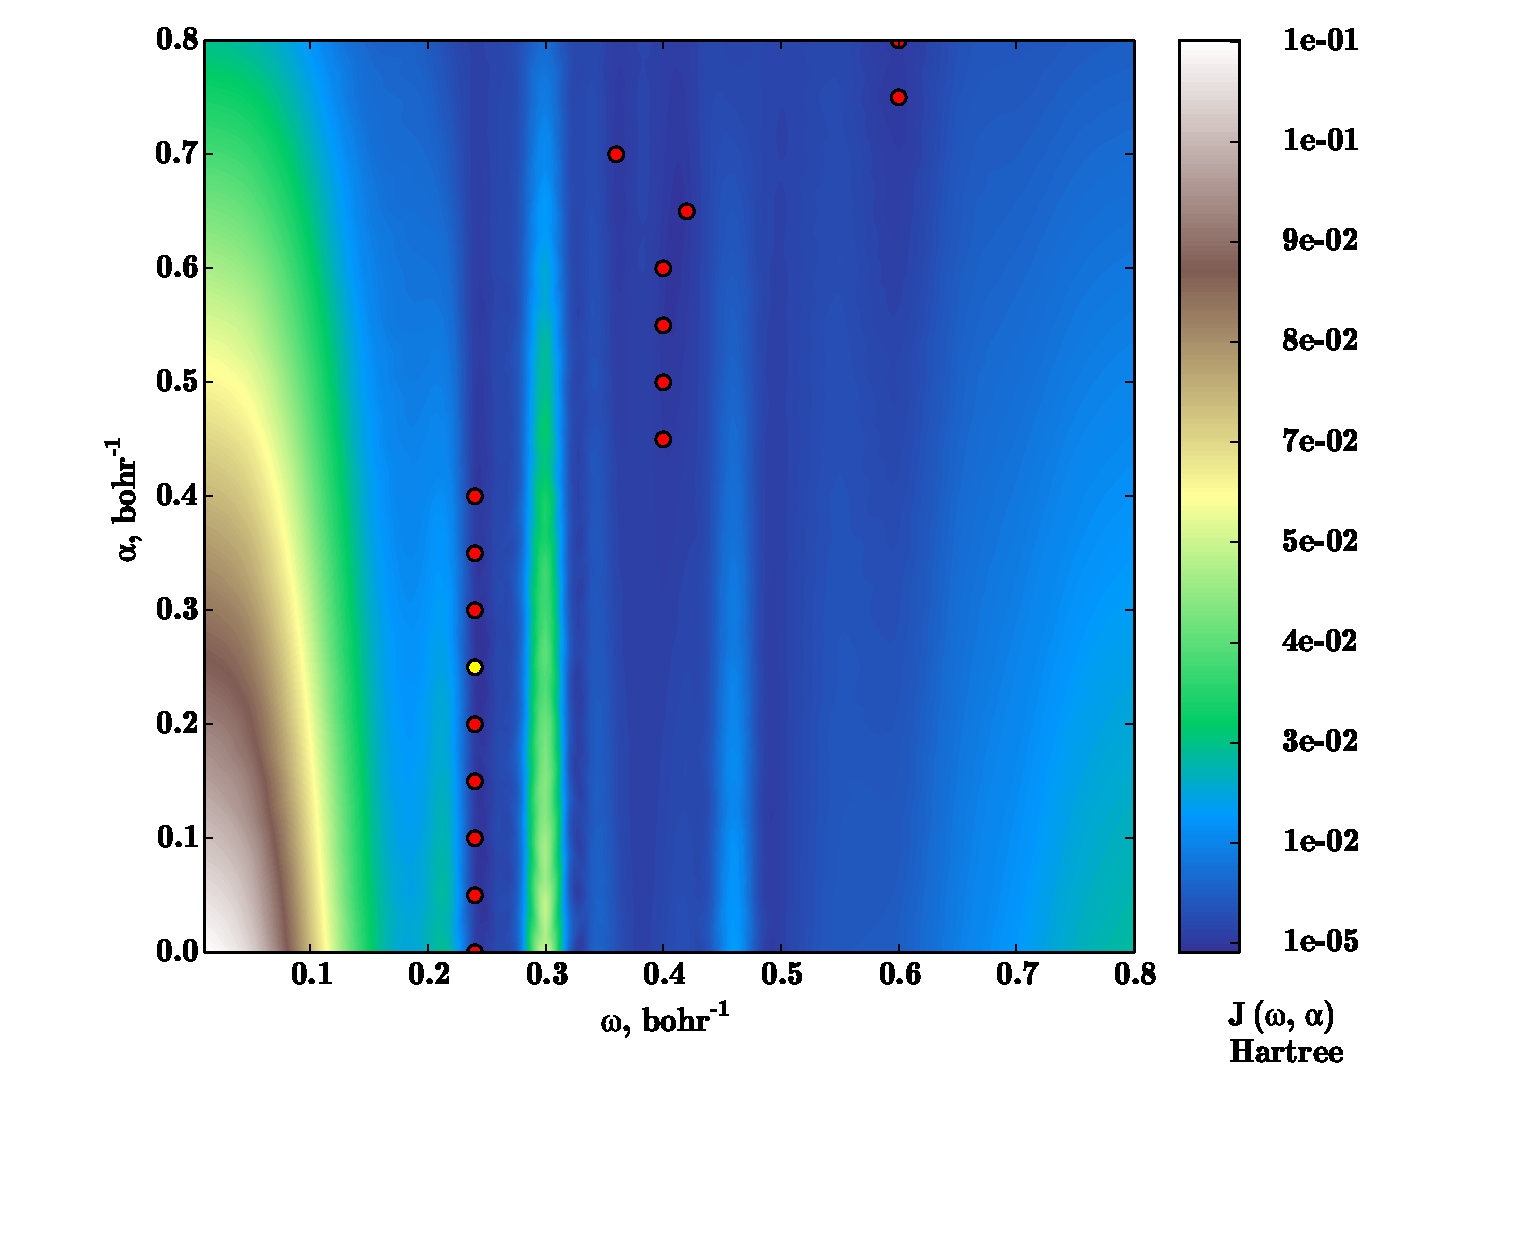
\includegraphics[width=0.69\textwidth]{Figures/Lithium/Lithium_J0_2D_terrain_path_spline_cut}
\label{fig:Lith-otrsh}
\caption{The functional $J(\alpha,\omega)$ described in eqation (\ref{eq:J_ao}) for Lithium}
\end{wrapfigure}

The appearance of $2p$-states are accessed by a dipole-transition in the bound part and can not be described within the theory applied here due to the neglect of the conjugate DO term in equation (\ref{eq:fullDO}) \cite{saPonzi}.

\section{Triatomic Linear Molecules}
There are several studies on CO$_2$ \cite{CO2, CO2_highres, HighResLinear, DiffLinear}, CS$_2$ \cite{DiffLinear,HighResLinear}, COS \cite{DiffLinear,HighResLinear} and N$_2$O \cite{DiffLinear}

CS$_2$ is known to have strong correlation effects \cite{2phcederbaum}

\section{water}
The PES and threshold PES, where the kinetic energy of the photoelectron is kept constant instead of the energy of the photon, of water is experimentally well studied 
for different photon energies.
As example, in Ref. \cite{waterTPE} the PES of water and several TPES of water and heavy water are investigated with high resolution.\\
Similar high accuracy is achieved in Ref. \cite{waterHePES} where the PES of H$_2$O$^+$ and D$_2$O$^+$ are studied with a He1 source, radiating at $537\,$Angs.\\
Further PES are available at higher photon energies:
In \cite{water1200}, photons at energies of $1200\,$eV are used.
A further study of Winter \textit{et. al.} measured spectra at $60$, $75$ $80$, $100$ and $120\,$eV in gas and liquid phase \cite{winterWater}.\\
These studies are of interest here since they yield a variety of different test-cases on a single system that can be used to prove the method being used to be valid.
